\documentclass[12pt]{article}

\usepackage{lipsum}     % 生成随机文字
\usepackage{graphicx}
\usepackage{booktabs}

\usepackage{geometry}   % 设置页边距
\geometry{a4paper, hmargin=2.54cm, vmargin=3.18cm}

\usepackage{setspace}   % 设置行距
\onehalfspacing         % 1.5 倍行距

% 设置表格格式
\usepackage{array}
\renewcommand{\arraystretch}{1.2} % 基础行距
\setlength{\defaultaddspace}{3pt} % booktabs默认间距

% 去掉图/表编号与题注文字之间的冒号，改为两个空格
\usepackage{caption}
\DeclareCaptionLabelSeparator{twospace}{~~}
\captionsetup{labelsep=twospace}

% 设置图编号格式：节编号.序号
\makeatletter 
\@addtoreset{figure}{section} 
\makeatother 
\renewcommand{\thefigure}{\arabic{section}.\arabic{figure}} 

% 设置表编号格式：节编号.序号
\makeatletter 
\@addtoreset{table}{section} 
\makeatother 
\renewcommand{\thetable}{\arabic{section}.\arabic{table}} 

% 一般最后调用 hyperref 宏包
% 思考1：对比 colorlinks, hidelinks 选项，超链接文字有怎样的不同？
\usepackage[colorlinks]{hyperref}


\begin{document}
    \tableofcontents
    
    \section{Hyperlinks in \LaTeX}
    
    Click \href{https://www.bilibili.com/}{here} to start your trip in Bilibili!

    
    \section{Table in \LaTeX}

    \lipsum[1]

    As shown in Table~\ref{tab:Univ-rank-2024} in page \pageref{tab:Univ-rank-2024}.

    % \usepackage{booktabs}
    \begin{table}[htbp]
        \centering
        \caption{Chinese Universities Ranked in the Top 50 in QS 2024}
        \label{tab:Univ-rank-2024}
        \begin{tabular}{@{}ccc@{}}
        \toprule
        Rank & University Name                               & Location         \\ \midrule
        17   & Peking University                             & China (Mainland) \\
        25   & \textbf{Tsinghua University}                  & China (Mainland) \\
        44   & Zhejiang University                           & China (Mainland) \\
        50   & Fudan University                              & China (Mainland) \\
        \bottomrule
        \end{tabular}
    \end{table}

    \lipsum[2]


    \section{Image in \LaTeX}

    \lipsum[3]

    As shown in Figure~\ref{fig:starryNight}        % 标签序号
    in the page \pageref{fig:starryNight}.          % 标签所在页码

% 思考2：尝试将浮动体位置选项改为 强制位于此处（H）（需要在导言区调用 float 宏包）
    \begin{figure}%[htbp]   % 默认选项是 t-b-p
        \centering
        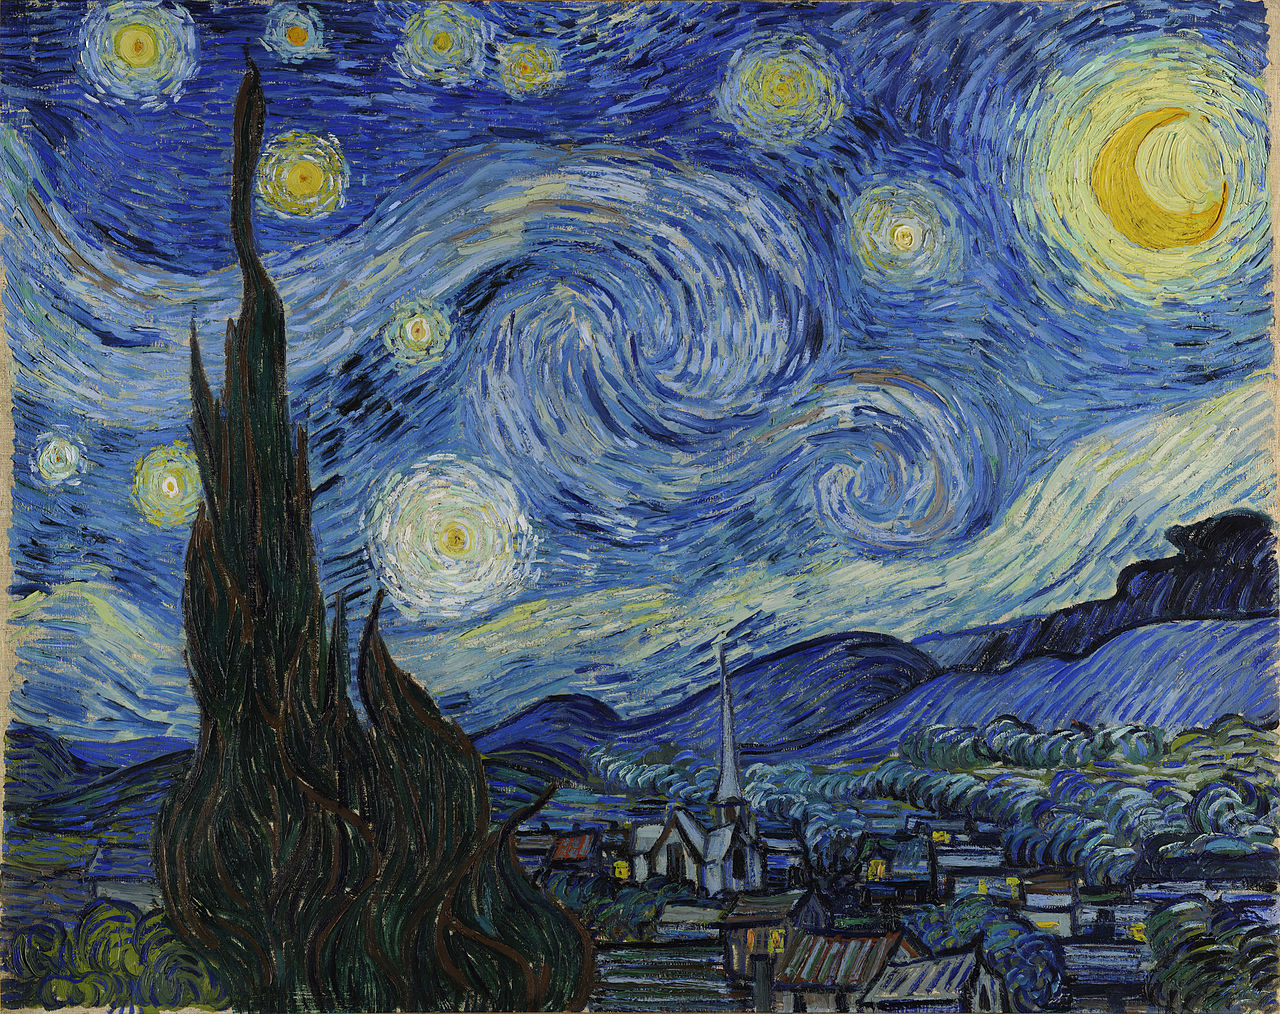
\includegraphics[width=0.6\linewidth]{figures/starryNight.jpg}
        \caption{A figure of starry night by Vincent}
        \label{fig:starryNight}
    \end{figure}

    \lipsum[4]
    

\end{document}